\section{Problema y algoritmos de filtraje}
Se considera un sistema controlado-observado estocástico a tiempo discreto
\begin{align*}
	\mathbf{x}_{k+1} &= \mathbf{f}(t_k, \mathbf{x}_k, \mathbf{u}_k, \mathbf{w}_k) \\
	\mathbf{y}_k &= \mathbf{g}(t_k, \mathbf{x}_k, \mathbf{u}_k, \mathbf{v}_k)
\end{align*}
Donde:
\begin{itemize}
	\item $\mathbf{f}: \R \times \R^{n_x} \times \R^{n_u} \times \R^{n_w} \to \R^{n_x}$ es la función de dinámica.
	\item $\mathbf{g}: \R \times \R^{n_x} \times \R^{n_u} \times \R^{n_v} \to \R^{n_y}$ es la función de observación
\end{itemize}
Siendo $n_x$ la dimensión del estado, $n_y$ la dimensión de la observación, $n_u$ la dimensión del \textit{input}, $n_w$ la dimensión del proceso estocástico en la dinámica y $n_v$ la dimensión del ruido en las observaciones. Se considera una condición inicial $\mathbf{x}_0$, por lo general desconocida sobre la que se coloca un \textit{prior} $X_0$. \\
Se supondrá que tanto $\mathbf{v}_k$ como $\mathbf{w}_k$ son vectores aleatorios centrados tal que $\mathbf{w}_k \indep \mathbf{w}_m, \, \forall k \neq m$, $\mathbf{v}_k \indep \mathbf{v}_m, \, \forall k \neq m$ y $\mathbf{w}_k \indep \mathbf{v}_k, \, \forall k$. Diremos que $\mathbf{w}$ y $\mathbf{v}$ son la perturbación en la dinámica y ruido en la medición, respectivamente. \\
El estudio de sistemas a tiempo continuo, formulados como
\begin{align*}
	\mathbf{x}'(t) &= \mathbf{f}(t, \mathbf{x}(t), \mathbf{u}(t), \mathbf{w}(t)) \\
	\mathbf{y}(t) &= \mathbf{g}(t, \mathbf{x}(t), \mathbf{u}(t), \mathbf{v}(t))
\end{align*}
muchas veces se reduce al caso discreto con esquemas de tipo Euler, por lo que durante esta tesis se mantendrá el foco en sistemas a tiempo discreto, a menos de que se necesite lo contrario. \\
El objetivo en el caso discreto será, en un instante $k$ encontrar un estimador de $\mathbf{x}_{k+\alpha}$, en base a observaciones $\{\Tilde{\mathbf{y}}_k\}_k$, que será denotado por $\hat {\mathbf{x}}_{k+\alpha}$. Dependiendo del valor de $\alpha$ el algoritmo recibirá una categoría diferente:
\begin{itemize}
	\item Predicción: $\alpha > 0$.
	\item Filtraje: $\alpha = 0$.
	\item Suavizado: $\alpha < 0$.
\end{itemize}
Así también se denotará a $\hat {\mathbf{x}}_{k_1|k_2}$ a la estimación del estado en la iteración $k_1$ dadas mediciones hasta la iteración $k_2$, entonces se dirá que $\hat{\mathbf{x}}_{k_1 | k_2}$ es un estado
\begin{itemize}
	\item Suavizado, si $k_2 > k_1$ ($t_2 > t_1$).
	\item Filtrado, si $k_2 = k_1$ ($t_2 = t_1$).
	\item Predicho, si $k_1 > k_2$ ($t_1 > t_2$).
\end{itemize}
El caso del filtraje será el centro durante este trabajo. Un algoritmo de filtraje busca estimar en el tiempo presente el estado en base a observaciones ruidosas, que puede ser entendido como el primer proceso en la estimación del estado de un sistema. \\
Posterior al filtraje de una medición ruidosa, se siguen los procesos de predicción y/o suavizado, siendo el primero la tarea poder estimar estados futuros en base al pasado, sin información del momento a estimar. Mientras que el suavizado es la capacidad de estimar momentos pasados, lo que se utiliza para mejorar las estimaciones presentes.\\
Se denota por $\mathbf{y}_{1:k}$, $\mathbf{u}_{0:k}$ a las observaciones e \textit{inputs}, respectivamente, hasta el tiempo $k \in \N$, a $k \in \N$ le llamaremos el horizonte del problema.  Notar que se considerará que no se tiene una observación de la condición inicial.\\ 
El problema de filtraje se puede formular como un problema de optimización del error cuadrático medio de la estimación, condicional a las observaciones y a los \textit{inputs}
\begin{equation*}
	(P) \quad
	\begin{cases}
		\begin{aligned}
			\text{mín} \quad & \quad \sum_{k=0}^N \E \left [ (\hat{\mathbf{x}}_{k|k} - \mathbf{x}_k)^T(\hat{\mathbf{x}}_{k|k} - \mathbf{x}_k) | \mathbf{y}_{0:k}, \, \mathbf{u}_{0:k}  \right] \\ 
			\text{s.a} \quad & \quad \mathbf{x}_{k+1} = \mathbf{f}(t_k, \mathbf{x}_k, \mathbf{u}_k, \mathbf{w}_k) \\
			\text{} \quad & \quad \mathbf{y}_k = \mathbf{g}(t_k, \mathbf{x}_k, \mathbf{u}_k, \mathbf{v}_k) \\
			\text{} \quad & \quad \mathbf{x}_0 \sim X_0
		\end{aligned}
	\end{cases}
\end{equation*}
Es entonces que el problema $(P)$ tiene como solución al estimador de mínimo error cuadrático. Es sabido de \cite{Kalman1960AProblems, Setoodeh2022NonlinearApplications} que este problema tiene un óptimo global dado por la esperanza condicional, que coincide con la noción de dicho estimador.
\begin{prop}
	El óptimo de $(P)$ viene dado por 
	\begin{equation*}
		\hat{\mathbf{x}}_{k|k} = \E \left [ \mathbf{x}_k | \mathbf{y}_{1:k}, \, \mathbf{u}_{0:k}  \right], \quad \forall k \in \{ 0, \dots, N \}
	\end{equation*}
\end{prop}
\noindent Aunque dicha cantidad no sea computable por métodos clásicos, como Monte Carlo, existen algoritmos para poder calcularla tiempo a tiempo, aunque sea de manera aproximada. 
\subsection{Caso a tiempo discreto, dinámica lineal y ruido centrado}
Para abordar el caso de sistemas dinámicos controlados-observados generales, es importante estudiar primero el caso lineal y con ruidos centrados y segundo momento finito, esto es
\begin{equation}
	\begin{cases}
		\mathbf{x}_{k+1} &= \mathbf{A}_k \mathbf{x}_k + \mathbf{B}_k \mathbf{u}_k + \mathbf{v}_k \\
		\mathbf{y}_k &= \mathbf{C}_k \mathbf{x}_k + \mathbf{D}_k \mathbf{u}_k  + \mathbf{w}_k
	\end{cases}
	\label{eq:lin_disc}
\end{equation}
con $\mathbf{A}_k \in \R^{n_x \times n_x}$, $\mathbf{B}_k \in \R^{n_x \times n_u}$, $\mathbf{C}_k \in \R^{n_y \times n_x}$, $\mathbf{D}_k \in \R^{n_y \times n_u}$,  $\mathbf{v}_k \sim \mathcal{N}(0, \mathbf{Q}_k)$ y $\mathbf{w}_k \sim \mathcal{N}(0, \mathbf{R}_k)$, $\mathbf{Q}_k \in \R^{n_x \times n_x}$, $\mathbf{R}_k \in \R^{n_y \times n_y}$. matrices de covarianzas, se tiene un algoritmo muy utilizado en ingeniería y ciencia, con suficiente fundamentos matemáticos e implementaciones eficientes, denotado el filtro de Kalman en honor a Rudolf E. Kalman, quién propuso el algoritmo por primera vez en \cite{Kalman1960AProblems}. Los detalles del algoritmo se presentan en el pseudo-código del Algoritmo \ref{alg:KF}. \\
\begin{algorithm}
	\caption{Filtro de Kalman}\label{alg:KF}
	\begin{algorithmic}[1]
		\State \textbf{Entrada:} Dinámica discreta como en (\ref{eq:lin_disc}), $\mathbf{x}_0$ \textit{prior} sobre la condición inicial, $\mathbf{y}_{1:N}$ observaciones, $\mathbf{u}_{0:N}$ \textit{inputs}.
		\State \textbf{Salida:} $(\hat{\mathbf{x}}_{k|k})_{k=0}^{N}$ estimador de la trayectoria y $(\hat{\mathbf{P}}_{k|k})_{k=0}^{N}$ matrices de covarianza.
		\State $\hat{\mathbf{x}}_{0|0}   \gets \E [\mathbf{x}_0]$
		\State $\mathbf{P}_{0|0} \gets \E [(\mathbf{x}_0 - \hat{\mathbf{x}}_{0})(\mathbf{x}_0 - \hat{\mathbf{x}}_{0})^T]$
		\For{$k = 0, \dots, N-1$}
		\State $\hat{\mathbf{x}}_{k+1|k} \gets \mathbf{A}_k \mathbf{x}_{k|k} + \mathbf{B}_k \mathbf{u}_k$
		\Comment{Estimación a priori}
		\State $\mathbf{P}_{k+1|k} \gets \mathbf{A}_k \mathbf{P}_{k|k} \mathbf{A}_k^T + \mathbf{Q}_k$
		\Comment{Error de covarianza a priori}
		\State $\hat{\mathbf{y}}_{k+1|k} \gets \mathbf{C}_{k+1} \hat{\mathbf{x}}_{k+1|k}$ 
		\Comment{Estimación de observación a priori}
		\State $\mathbf{e}_{\mathbf{y}_{k+1|k}} \gets \mathbf{y}_{k+1} - \hat{\mathbf{y}}_{k+1|k}$
		\Comment{Error a priori (innovación)}
		\State $\mathbf{K}_{k+1} \gets \mathbf{P}_{k+1|k} \mathbf{C}^T_{k+1} (\mathbf{C}_{k+1} \mathbf{P}_{k|k} \mathbf{C}^T_{k+1}+ \mathbf{R}_{k+1})^{-1}$
		\Comment{Ganancia de Kalman}
		\State $\hat{\mathbf{x}}_{k+1|k+1} \gets \hat{\mathbf{x}}_{k+1|k} + \mathbf{K}_{k+1} \mathbf{e}_{\mathbf{y}_{k+1|k}}$
		\Comment{Error a posteriori}
		\State $\mathbf{P}_{k+1|k+1} \gets (\mathbf{I} - \mathbf{K}_{k+1} \mathbf{C}_{k+1}) \mathbf{P}_{k+1|k}$
		\Comment{Error de covarianza a posteriori}
		\EndFor
	\end{algorithmic}
\end{algorithm}\\
El siguiente resultado le da toda su validez al algoritmo del Filtro de Kalman, que es probado en el artículo original \cite{Kalman1960AProblems}.
\begin{prop}
	El algoritmo del filtro de Kalman devuelve una secuencia $(\hat{\mathbf{x}}_{k|k})_k$ tal que 
	\begin{equation*}
		\hat{\mathbf{x}}_{k|k} = \E \left [ \mathbf{x}_k | \mathbf{y}_{1:k}, \, \mathbf{u}_{0:k}  \right], \quad \forall k \in \{ 0, \dots, N \}
	\end{equation*}
\end{prop}
\noindent Como consecuencia del hecho de que en el contexto Gaussiano el estimador de mínimo error cuadrático medio coincide con el estimador de máximo a posteriori, se tiene el siguiente resultado.
\begin{prop}
	El algoritmo del filtro de Kalman devuelve una secuencia $(\hat{\mathbf{x}}_{k|k})_k$ tal que 
	\begin{equation*}
		\hat{\mathbf{x}}_{k|k} \in \arg \max_{\hat{\mathbf{x}}_{k|k}} p (\hat{\mathbf{x}}_{k|k} | \mathbf{y}_{1:k}, \, \mathbf{u}_{0:k})
	\end{equation*}
\end{prop}

\subsection{Caso a tiempo discreto no lineal general}
A diferencia del caso anterior, en el caso no lineal general hay muchos algoritmos propuestos, siendo los más clásicos las variantes del filtro de Kalman, como el \textit{Extended Kalman Filter} (EKF) y el \textit{Unscented Kalman Filter} (UKF), pero se sabe que resultan ser subóptimos \cite{Setoodeh2022NonlinearApplications}.\\ 
A pesar de que dichos algoritmos reciben dinámicas no lineales, siguen suponiendo que el ruido es aditivo, centrado y Gaussiano. Se verá en secciones posteriores que esto no es un impedimento para poder ejecutarlos, pero una familia de métodos se han construido para el caso más general, cuyos representantes más famosos son los filtros de partículas.\\
Con el motivo de no extender más este informe solo se expondrá el algoritmo de EKF. Para esta sección se supondrá que la dinámica es de la forma
\begin{equation}
	\begin{aligned}
		\mathbf{x}_{k+1} &= \mathbf{f}(t_k, \mathbf{x}_k, \mathbf{u}_k) + \mathbf{w}_k \\
		\mathbf{y}_k &= \mathbf{g}(t_k, \mathbf{x}_k, \mathbf{u}_k) + \mathbf{v}_k 
	\end{aligned}
	\label{eq:no_lin_disc_add}
\end{equation}
Con $\mathbf{w}_k \sim \mathcal{N}(0, \mathbf{Q}_k)$ y $\mathbf{v}_k \sim \mathcal{N}(0, \mathbf{R}_k)$. 
El algoritmo de \textit{Extended Kalman Filter}, cuyo pseudo-código puede visualizarse en el algoritmo \ref{alg:EKF}, busca linearizar el sistema a primer orden vía su Jacobiano, tanto para $\mathbf{f}$ como para $\mathbf{g}$ de manera de generar las matrices $\mathbf{A}_k$ y $\mathbf{C}_k$ necesarias para el Filtro de Kalman, respectivamente. \\
A pesar de los simple que parece la adaptación de este algoritmo al caso no lineal, ilustra que extender el filtro de Kalman al caso no lineal se basa en una linealización de la dinámica, en este caso vía Jacobiano, pero podrían existir otras, que es en lo que se basará el filtro creado durante este trabajo.

\begin{algorithm}
	\caption{\textit{Extended Kalman Filter}}\label{alg:EKF}
	\begin{algorithmic}[1]
		\State \textbf{Entrada:} Dinámica discreta como en (\ref{eq:no_lin_disc_add}), $\mathbf{x}_0$ \textit{prior} sobre la condición inicial,  $\mathbf{y}_{1:N}$ observaciones, $\mathbf{u}_{0:N}$ \textit{inputs}.
		\State \textbf{Salida:} $(\hat{\mathbf{x}}_{k|k})_{k=0}^{N}$ estimador de la trayectoria y $(\hat{\mathbf{P}}_{k|k})_{k=0}^{N}$ matrices de covarianza.
		\State $\hat{\mathbf{x}}_{0|0}   \gets \E [\mathbf{x}_0]$
		\State $\mathbf{P}_0 \gets \E [(\mathbf{x}_0 - \hat{\mathbf{x}}_{0})(\mathbf{x}_0 - \hat{\mathbf{x}}_{0})^T]$
		\For{$k = 0, \dots, N-1$}
		\State $\mathbf{A}_k \gets \nabla _\mathbf{x} \mathbf{f} (t_k, \hat{\mathbf{x}}_{k|k}, \mathbf{u}_k)$
		\Comment{Linealización de la función de dinámica}
		
		\State $\hat{\mathbf{x}}_{k+1|k} \gets \mathbf{f}(t_k, \hat{\mathbf{x}}_{k|k}, \mathbf{u}_k)$
		\Comment{Estimación a priori}
		\State $\mathbf{P}_{k+1|k} \gets \mathbf{A}_k \mathbf{P}_{k|k} \mathbf{A}_k^T + \mathbf{Q}_k$
		\Comment{Error de covarianza a priori}
		\State $\mathbf{C}_{k+1} \gets \nabla_\mathbf{x} \mathbf{g} (t_k, \hat{\mathbf{x}}_{k+1|k}, \mathbf{u}_k)$
		\Comment{Linealización de la función de observación}
		\State $\hat{\mathbf{y}}_{k+1|k} \gets \mathbf{g}(t_k, \hat{\mathbf{x}}_{k+1|k}, \mathbf{x}_{k+1})$ 
		\Comment{Estimación de observación a priori}
		\State $\mathbf{e}_{\mathbf{y}_{k+1|k}} \gets \mathbf{y}_{k+1} - \hat{\mathbf{y}}_{k+1|k}$
		\Comment{Error a priori (innovación)}
		\State $\mathbf{K}_{k+1} \gets \mathbf{P}_{k+1|k} \mathbf{C}^T_{k+1} (\mathbf{C}_{k+1} \mathbf{P}_{k|k} \mathbf{C}^T_{k+1} + \mathbf{R}_{k+1})^{-1}$
		\Comment{Ganancia de Kalman}
		\State $\hat{\mathbf{x}}_{k+1|k+1} \gets \hat{\mathbf{x}}_{k+1|k} + \mathbf{K}_{k+1} \mathbf{e}_{y_{k+1|k}}$
		\Comment{Error a posteriori}
		\State $\mathbf{P}_{k+1|k+1} \gets (\mathbf{I} - \mathbf{K}_{k+1} \mathbf{C}_{k+1}) \mathbf{P}_{k+1|k}$
		\Comment{Error de covarianza a posteriori}
		\EndFor
	\end{algorithmic}
\end{algorithm}

El algoritmo del \textit{Unscented Kalman Filter} (UKF), pseudo-código del algoritmo \ref{alg:UKF}, se basa en generar puntos de muestra (llamados puntos sigma) alrededor de la estimación actual del estado del sistema. Estos puntos permiten representar la distribución estadística de la estimación sin necesidad de calcular derivadas. Al propagar estos puntos sigma a través del modelo no lineal, el UKF logra realizar estimaciones en el siguiente instante de tiempo, capturando de manera precisa las propiedades no lineales del sistema. Esta estrategia hace que el UKF sea una alternativa robusta al \textit{Extended Kalman Filter} (EKF) para el seguimiento y la estimación en sistemas no lineales. Aún así, el algoritmo puede ser costoso en la práctica y es necesaria una gran cantidad de puntos sigma para lograr una estimación fiable.

\begin{algorithm}[h!]
	\caption{\textit{Unscented Kalman Filter}}\label{alg:UKF}
	\begin{algorithmic}[1]
		\State \textbf{Entrada:} Dinámica discreta como en (\ref{eq:no_lin_disc_add}), $\mathbf{x}_0$ \textit{prior} sobre la condición inicial,  $\mathbf{y}_{1:N}$ observaciones, $\mathbf{u}_{0:N}$ \textit{inputs}.
		\State \textbf{Salida:} $(\hat{\mathbf{x}}_{k|k})_{k=0}^{N}$ estimador de la trayectoria y $(\hat{\mathbf{P}}_{k|k})_{k=0}^{N}$ matrices de covarianza.
		
		\State \textbf{Inicialización:}
		\State $\hat{\mathbf{x}}_{0|0}   \gets \E [\mathbf{x}_0]$
		\State $\mathbf{P}_0 \gets \E [(\mathbf{x}_0 - \hat{\mathbf{x}}_{0})(\mathbf{x}_0 - \hat{\mathbf{x}}_{0})^T]$
		
		\For{$k = 1, 2, \dots, N$}
		
		\State Calcular los puntos sigma $\chi$ usando la estimación del estado actual $\hat{\mathbf{x}}_{k-1}$ y la covarianza $\mathbf{P}_{k-1}$. Asignar pesos a los puntos sigma de acuerdo con pesos predefinidos $W_m$ (para la media) y $W_c$ (para la covarianza).
		
		\State $\chi_{k|k-1}^{(i)} \gets \mathbf{f}(t_k, \chi_{k-1}^{(i)}, \mathbf{u}_k)$
		\Comment Propagar cada punto sigma a través de la dinámica.
	
		\State $\hat{\mathbf{x}}_{k|k-1} \gets \sum_{i} W_m^{(i)} \chi_{k|k-1}^{(i)}$
		\Comment Calcular la media del estado predicho.
		
		\State Calcular la covarianza predicha:
		\[
		\mathbf{P}_{k|k-1} = \sum_{i} W_c^{(i)} \left( \chi_{k|k-1}^{(i)} - \hat{\mathbf{x}}_{k|k-1} \right) \left( \chi_{k|k-1}^{(i)} - \hat{\mathbf{x}}_{k|k-1} \right)^\top + \mathbf{Q}_k
		\]
		
		\State $\gamma_{k}^{(i)} = \mathbf{h}(t_k, \chi_{k|k-1}^{(i)}, \mathbf{u}_k)$
		\Comment{Pasar cada punto sigma predicho a través de la observación.}
		
		\State $\hat{\mathbf{y}}_k = \sum_{i} W_m^{(i)} \gamma_{k}^{(i)}$
		\Comment{Calcular la media de la medición predicha.}
		\State Calcular la covarianza de la medición:
		\[
		 \mathbf{S}_k = \sum_{i} W_c^{(i)} \left( \gamma_{k}^{(i)} - \hat{ \mathbf{y}}_k \right) \left( \gamma_{k}^{(i)} - \hat{\mathbf{y}}_k \right)^\top + \mathbf{R}_k
		\]
		\State Calcular la covarianza cruzada:
		\[
		\mathbf{C}_k = \sum_{i} W_c^{(i)} \left( \chi_{k|k-1}^{(i)} - \hat{\mathbf{x}}_{k|k-1} \right) \left( \gamma_{k}^{(i)} - \hat{\mathbf{x}}_k \right)^\top
		\]

		\State $\mathbf{K}_k = \mathbf{C}_k \mathbf{S}_k^{-1}$
		\Comment{Calcular la ganancia de Kalman.}
		\State $\hat{ \mathbf{x}}_{k|k} = \hat{ \mathbf{x}}_{k|k-1} +  \mathbf{K}_k ( \mathbf{y}_k - \hat{ \mathbf{y}}_k)$ 
		\Comment{Actualizar la estimación del estado.}
		\State $\mathbf{P}_{k|k} =  \mathbf{P}_{k|k-1} -  \mathbf{K}_k \mathbf{S}_k  \mathbf{K}_k^\top$
		\Comment{Actualizar la covarianza.}
		
		\EndFor
		
	\end{algorithmic}
\end{algorithm}

Los Filtros de Partículas (PF) o algoritmos de \textit{Sequential Monte Carlo} (SMC) \cite{Kemp2003AnMethods, Wills2023SequentialReview} son una familia de métodos que estiman el estado de sistemas dinámicos no lineales y/o no gaussianos mediante técnicas de muestreo tipo Monte Carlo. Estos algoritmos representan la distribución de probabilidad del estado mediante un conjunto de partículas, que son muestras aleatorias ponderadas según su probabilidad. La precisión de estos filtros depende críticamente del proceso de resampling, un paso fundamental que evita la degeneración de partículas al eliminar aquellas con pesos bajos y duplicar las más probables. Esto permite que los filtros de partículas mantengan una representación precisa de la distribución posterior en cada paso de tiempo, adaptándose dinámicamente a la complejidad del sistema.
Para el algoritmo se considerará que los modelos vienen representados por distribuciones de probabilidad, una de transición para la dinámica  \( p(\mathbf{x}_k | \mathbf{x}_{k-1}) \) y para la observación \( p(\mathbf{y}_k | \mathbf{x}_k) \).

\begin{algorithm}[h!]
	\caption{Filtro de Partículas}
	\begin{algorithmic}[1]
		
		\State \textbf{Entrada:} Modelo de dinámica \( p(\mathbf{x}_k | \mathbf{x}_{k-1}) \), modelo de medición \( p(\mathbf{y}_k | \mathbf{x}_k) \), observaciones \( \mathbf{y}_{1:k} \), número de partículas \( N_p \), estado inicial \( \{ \mathbf{x}_0^{(i)} \}_{i=1}^{N_p} \)
		\State \textbf{Salida:} Estimación del estado basada en la distribución ponderada de partículas \( \{ \mathbf{x}_k^{(i)}, w_k^{(i)} \}_{i=1}^{N_p} \)
		
		\For{$i = 1, \dots, N_p$}
		\State Generar la partícula inicial \( \mathbf{x}_0^{(i)} \) de la distribución inicial \( p(\mathbf{x}_0) \)
		\State Asignar el peso inicial \( w_0^{(i)} = \frac{1}{N_p} \)
		\EndFor
		
		\For{$k = 1, 2, \dots, N$}
		
		\For{$i = 1, \dots, N_p$}
		\State Muestrear \( \mathbf{x}_k^{(i)} \sim p(\mathbf{x}_k | \mathbf{x}_{k-1}^{(i)}) \) \Comment{Propagar cada partícula por la dinámica.}
		\EndFor
		
		\For{$i = 1, \dots, N_p$}
		\State \( w_k^{(i)} = w_{k-1}^{(i)} \cdot p(\mathbf{y}_k | \mathbf{x}_k^{(i)}) \) \Comment{Actualizar peso basado en la observación.}
		\EndFor
		
		\State \( w_k^{(i)} = \frac{w_k^{(i)}}{\sum_{j=1}^{N_p} w_k^{(j)}} \)
		\Comment{Normalizar los pesos.}
		
		\If{la degeneración de partículas es alta}
		\State Re-samplear las partículas \( \{ \mathbf{x}_k^{(i)}, w_k^{(i)} \}_{i=1}^{N_p} \) según sus pesos \( w_k^{(i)} \)
		\State Reiniciar pesos: \( w_k^{(i)} = \frac{1}{N_p} \) para todas las partículas
		\EndIf
		
		\EndFor
		
	\end{algorithmic}
\end{algorithm}

Un aspecto importante de los Filtros de Partículas es que su orden de convergencia ha sido demostrado como $O(N_p^{-1/2})$ \cite{Crisan2002APractitioners, Chopin2020AnCarlo}, es decir, la precisión del método aumenta proporcionalmente a la raíz cuadrada inversa del número de partículas utilizadas. Este número de partículas, que se elige como parámetro del filtro, controla directamente el error de estimación. Esta cota de error se tomará como referencia de comparación en el presente trabajo.

% RKHS
\section{Reproducing Kernel Hilbert Spaces}
Esta sección se basa en \cite{Wendland2004ScatteredApproximation} y \cite{Berlinet2004ReproducingStatistics}, aunque una versión más moderna de los resultados se puede encontrar en \cite{Saitoh2016TheoryApplications}. Sea \( \X \) un espacio topológico, y denote \(\C^\X\) al espacio de todas las funciones de \( \X \) en los números complejos. 

\begin{defn}[Reproducing Kernel Hilbert Space (RKHS)]  
Un espacio de Hilbert \( \mathcal{H} \subset \C^\X \) se dice un RKHS si existe una función \( k: \X \times \X \to \C \), llamada \textit{kernel reproduciente}, tal que:
\begin{enumerate}
    \item \( k_p \equiv K(\cdot, p) \in \mathcal{H}, \, \forall p \in E \).
    \item \( f(p) = \langle f, k_p \rangle_{\mathcal{H}}, \quad \forall p \in E, \, \forall f \in \mathcal{H}. \)
\end{enumerate}
\end{defn}

\noindent La segunda propiedad, conocida como \textit{propiedad reproduciente}, es fundamental en la teoría de los RKHS y da paso a muchas de las propiedades relevantes en estos espacios, como aquellas que se presentarán a continuación. Denotamos por \( \mathcal{H}_K(E) \) al espacio de Hilbert de funciones de \( E \) en \( \C \) cuyo kernel reproduciente es \( k \).

El siguiente lema proporciona una condición necesaria y suficiente para que un espacio de Hilbert dado posea un kernel reproduciente.

\begin{lema}
Un espacio de Hilbert \( \mathcal{H} \subset \C^\X \) posee un kernel reproduciente si y solo si los funcionales de evaluación \( e_p: \mathcal{H} \to \C \), definidos por \( e_p(f) = f(p) \), son continuos en \( \mathcal{H} \).
\end{lema}

\noindent Para construir un RKHS sobre un espacio topológico \( \X \), se introduce la siguiente definición.

\begin{defn}[Función semi-definida positiva]  
Una función \( k: \X \times \X \to \C \) se dice semi-definida positiva si para todo \( n \geq 1 \), \( (c_1, \dots, c_n) \in \C^n \), y \( (x_1, \dots, x_n) \in \X^n \), se cumple que:
\[
\sum_{i=1}^n \sum_{j=1}^n c_i \bar{c_j} K(x_i, x_j) \geq 0.
\]
\end{defn}

\noindent Esta propiedad es equivalente a que, para cada \( n \in \N \) y toda colección \( (x_1, \dots, x_n) \in \X^n \), la matriz  
\[
G = \left( k(x_i, x_j) \right)_{1 \leq i, j \leq n}
\]
sea Hermitiana y semi-definida positiva. Dicha matriz se denomina matriz Grammiana del kernel asociada a \( \{ x_i \}_{i=1}^n \), o simplemente matriz Grammiana cuando no haya lugar a confusión.

Finalmente, el siguiente lema describe cómo construir una función semi-definida positiva a partir de un espacio de Hilbert dado.

\begin{lema}
Sea \( \mathcal{H} \subset \C^\X \) un espacio de Hilbert con producto interno \( \langle \cdot, \cdot \rangle_\mathcal{H} \), y sea \( \varphi : \X \to \mathcal{H} \). Entonces, la función \( k: \X \times \X \to \C \), definida como
\[
k(x,y) = \langle \varphi(x), \varphi(y) \rangle_\mathcal{H},
\]
es semi-definida positiva.
\end{lema}

\noindent A continuación, dado un kernel \( k \) semi-definido positivo, se presentan un lema y un teorema que describen el comportamiento de un RKHS.

\begin{lema}
Sea \( \mathcal{H}_0 \) un subespacio de \( \C^\X \) en el cual se define un producto interno \( \langle \cdot, \cdot \rangle_{\mathcal{H}_0} \), con norma asociada \( \|\cdot\|_{\mathcal{H}_0} \). Entonces, para que exista un espacio de Hilbert \( \mathcal{H} \) tal que:
\begin{enumerate}
    \item[(1)] \( \mathcal{H}_0 \subset \mathcal{H} \subset \C^\X \), y la topología definida en \( \mathcal{H}_0 \) por el producto interno \( \langle \cdot, \cdot \rangle_{\mathcal{H}_0} \) coincida con la topología inducida en \( \mathcal{H}_0 \) por \( \mathcal{H} \),
    \item[(2)] \( \mathcal{H} \) posea un kernel reproduciente \( k \),
\end{enumerate}
es necesario y suficiente que:
\begin{enumerate}
    \item[(i)] Los funcionales de evaluación \( (e_t)_{t \in \X} \) sean continuos en \( \mathcal{H}_0 \),
    \item[(ii)] Cualquier sucesión de Cauchy \( (f_n) \) en \( \mathcal{H}_0 \) que converge puntualmente a cero, también converge a cero en el sentido de la norma.
\end{enumerate}
\end{lema}

\begin{teo}[Moore–Aronszajn \cite{Aronszajn1950TheoryKernels}]
Sea \( k \) una función semi-definida positiva en \( \X \times \X \). Entonces, existe un único espacio de Hilbert \( \mathcal{H} \subset \C^\X \) con \( k \) como kernel reproduciente. El subespacio \( \mathcal{H}_0 \) de \( \mathcal{H} \), generado por las funciones \( (k(\cdot, x))_{x \in \X} \), es denso en \( \mathcal{H} \), y \( \mathcal{H} \) coincide con el conjunto de funciones en \( \X \) que son límites puntuales de sucesiones de Cauchy en \( \mathcal{H}_0 \), con el producto interno definido por
\[
\langle f, g \rangle_{\mathcal{H}_0} = \sum_{i=1}^n \sum_{j=1}^m \alpha_i \bar{\beta}_j k(y_j, x_i),
\]
donde
\[
f(\cdot) = \sum_{i=1}^n \alpha_i k(\cdot, x_i), \quad g(\cdot) = \sum_{j=1}^m \beta_j k(\cdot, y_j),
\]
para \( (x_1, \dots, x_n) \in E^n \) y \( (y_1, \dots, y_m) \in \X^m \).
\end{teo}

\noindent El siguiente teorema permite transferir las propiedades de un RKHS a un espacio \( \ell^2 \), el cual resulta, en general, más sencillo de manipular.

\begin{teo}
Una función \( K: \X \times \X \to \C \) es un kernel reproduciente si y solo si existe una función \( \varphi: E \to \ell^2 (\Tilde{\X}) \), para algún espacio \( \ell^2(\Tilde{\X}) \), tal que para todo \( (x, y) \in \X \times \X \),
\[
k(x, y)= \langle \varphi(x), \varphi(y) \rangle_{\ell^2(\Tilde{\X})}.
\]
Además, el espacio \( \ell^2(\Tilde{\X}) \) es isométrico a \( \H_k(\X) \) a través de una isometría \( T: \X \to \ell^2(\Tilde{\X}) \), y la función \( \varphi \) viene dada por \( \varphi(x) = T(k(\cdot, x)) \). Dicha función \( \varphi \) se denomina el \textit{feature map} asociado a \( k \).
\end{teo}
En la literatura existen muchos kernels que son de utilidad en uno u otro contexto. A efectos de este trabajo se considerará el kernel de Matérn que, como se expondrá a lo largo de este escrito, posee muy buenas propiedades.
\begin{defn}
Se define el kernel de Matérn con parámetro de suavización \( \nu > 0 \) y ancho de banda \( \gamma > 0 \) como:
\[
k_{\nu}(x,y) = \frac{2^{1-\nu}}{\Gamma(\nu)} \left( \sqrt{2\nu} \frac{\|x-y\|}{\gamma} \right)^\nu B_\nu \left( \sqrt{2\nu} \frac{\|x-y\|}{\gamma} \right),
\]
donde \( \Gamma \) es la función Gamma y \( B_\nu \) es la función modificada de Bessel de segundo tipo de parámetro \( \nu \).

\end{defn}

El kernel de Matérn tiene una estrecha relación con los espacios de Sobolev fraccionarios, por lo que se introducen conceptos claves, como la definición de dicho espacio en $\R^d$ y la condición de cono interior.

\begin{defn}[Espacio de Sobolev fraccionario \cite{Adams2003SobolevSpaces}] Se define el espacio de Sobolev de regularidad $s > 0$ como
\[
H^s(\mathbb{R}^n) = \left\{ f \in L^2(\mathbb{R}^n) : \widehat{f}(\cdot)(1 + \|\cdot\|_2^2)^{s/2} \in L^2(\mathbb{R}^n) \right\},
\]
donde \( \widehat{f} \) denota la transformada de Fourier de \( f \).
\label{def:frac_sob}
\end{defn}

\begin{defn}[Condición de cono interior \cite{Wendland2004ScatteredApproximation}]
Un conjunto \( \Omega \subset \mathbb{R}^n \) satisface la condición del cono interior si existe un ángulo \( \theta \in (0, \pi/2) \) y un radio \( r > 0 \) tales que, para cada \( x \in \Omega \), existe \( \xi(x) \in \mathbb{R}^n \), con \( \|\xi(x)\|_2 = 1 \), de modo que el cono
\[
C(x, \xi(x), \theta, r) := \{x + \lambda y : y \in \mathbb{R}^n, \|y\| = 1, y^\top \xi(x) \geq \cos \theta, \lambda \in [0, r]\}
\]
está contenido en \( \Omega \).
\end{defn}
El siguiente teorema entrega una condición clave para los desarrollos de este trabajo, que es el hecho de que el kernel de Matérn es equivalente en norma a un espacio de Sobolev.
\begin{teo}[\cite{Wendland2004ScatteredApproximation, Tuo2016AProperties}]
Si \( \mathcal{X} \) es un conjunto compacto que satisface la condición del cono interior y \( k \) es el kernel de Matérn con parámetro \( \nu > 0 \), entonces para \( s = \nu + n/2 \) se cumple que \( \mathcal{H}_k (\mathcal{X}) \) es equivalente en norma a \( H^s (\mathcal{X}) \).
\end{teo}

\begin{obs}
    Si \( \nu = 1/2 \), se tiene que
\[
B_{1/2} (z) = \sqrt{ \frac{\pi}{2} } \frac{e^{-z}}{\sqrt{z}},
\]
por lo que se deduce que:
\[
\begin{aligned}
k (x,y) &= \frac{\sqrt{2}}{\Gamma(1/2)} \left(  \frac{\|x-y\|}{\gamma} \right)^{1/2} \sqrt{ \frac{\pi}{2} } \exp \left( -\frac{\|x-y\|}{\gamma} \right) \left(  \frac{\|x-y\|}{\gamma} \right)^{-1/2} = \exp \left( -\frac{\|x-y\|}{\gamma} \right).
\end{aligned}
\]
En consecuencia, el kernel de Matérn generaliza al kernel Laplace, y el RKHS asociado al kernel Laplace es \( H^{(n+1)/2} \).
\end{obs}
Notar que la definición \ref{def:frac_sob} no es válida cuando se tiene un subconjunto de $\R^n$, pero la deducción de esta propiedad en \cite{Wendland2004ScatteredApproximation} pasa por extender las funciones a todo $\R^n$ y luego aplicar la definición. \\
En las secciones posteriores será de interés hacer un \textit{embedding} de una distribución en un RKHS, para lo que es necesario definir el elemento medio en un RKHS y los operadores de covarianza. Las definiciones y proposiciones que siguen han sido expuestas en \cite{Fukumizu2004DimensionalitySpaces, Song2009HilbertSystems, Muandet2017KernelBeyond}. \\
Sean $\X \subset \R^n$, $\Y \subset \R^p$,  Sea $\mu$ una medida de probabilidad sobre $\X$, $\H$ un RKHS sobre $\X$ con kernel reproduciente $k$ y feature map $\Phi$ y $X$ una variable aleatoria con soporte en $\X$ y $Y$ una variable aleatoria con soporte en $\Y$.
\begin{defn}[Elemento medio \cite{Song2009HilbertSystems}]
	Se define el elemento medio en el RKHS $\H$ como
	
	\begin{equation*}
		\hat \mu = \int_\X \Phi (x) d \mu (x) \in \H
	\end{equation*}
\end{defn}
Se define el producto Kronecker en el contexto de RKHS como un operador multiplicativo y que generaliza el producto Kronecker de vectores.
\begin{defn}[Producto de Kronecker]
    El producto Kronecker en un RKHS se define como
    el siguiente operador de rango 1 para $x, y \in \X$ fijos
	$$ \Phi_\X (x) \otimes \Phi_\X(y) : \H_\X \to \H_\X$$
	\begin{equation*}
		[\Phi_\X (x) \otimes \Phi_\X(y)] \psi = \langle \psi, \Phi_\X (y) \rangle \Phi_\X (x) = \psi (y) \Phi_\X (x)
	\end{equation*}
    \label{def:kronecker}
\end{defn}
Notar que en la última igualdad se utilizó la propiedad reproduciente. Esto motiva la definición del operador de covarianza.
\begin{defn}[Operador de covarianza]
    El operador de covarianza asociado al \textit{feature map} $\Phi$ como $C_X : \H_\X \to \H_\X$ 
    \begin{equation*}
        C_X = \int_\X \Phi_\X (x) \otimes \Phi_\X (x) d \mu_\X (x)
    \end{equation*}
\end{defn}
La definición del operador de covarianza cruzada entre dos variables aleatorias será fundamental en el desarrollo posterior como embedding de las variables en un espacio de Hilbert.
\begin{defn}[Operador de covarianza cruzada]
    El operador de covarianza cruzada asociado a las variables aleatorias $X$ e $Y$ se define como el operador $C_{XY}: \H_\X \to \H_\Y$	
    \begin{equation*}
        C_{X Y} = \E [\Phi_\X (X) \otimes \Phi_\Y (Y)] = \int_\X \int_\Y \Phi_\X (x) \otimes \Phi_\Y (y) \rho_g (x, dy) d \mu_\X (x)
    \end{equation*}
\end{defn}

	El adjunto de estos operadores es sencillo de calcular
	\begin{prop}
		Sea $x \in \X$ e $y \in \Y$, luego
		
		\begin{equation*}
			\left ( \Phi_\X (x) \otimes \Phi_\Y (y) \right )^* = \Phi_\Y (y) \otimes \Phi_\X (x)
		\end{equation*}
	\end{prop}
	\begin{proof}
		Sean $h_\X \in \H_\X$, $h_\Y \in \H_\Y$, luego
		\begin{equation*}
			\langle (\Phi_\X (x) \otimes \Phi_\Y (y)) h_\Y, h_\X \rangle = \langle h_\Y (y) \Phi_\X (x), h_\X \rangle = h_\Y (y) \langle \Phi_\X (x), h_\X \rangle
		\end{equation*}
		Por propiedad reproduciente
		\begin{equation*}
			h_\Y (y) \langle  \Phi_\X (x), h_\X \rangle = h_\Y (y) h_\X (x)
		\end{equation*}
		A la vez
		\begin{equation*}
			\langle h_\Y, (\Phi_\Y (y) \otimes \Phi_\X (x)) h_\X \rangle = \langle h_\Y, h_\X (x) \Phi_\Y (y) \rangle = h_\X (x) 
			\langle h_\Y, \Phi_\Y (y) \rangle =
		\end{equation*}
		Nuevamente, por propiedad reproduciente
		\begin{equation*}
			h_\X (x) 
			\langle h_\Y, \Phi_\Y (y) \rangle =h_\X (x) h_\Y (y) 
		\end{equation*}
		Y se concluye lo pedido.
	\end{proof}
	
	\begin{cor} $(C_{X})^* = C_X$.
	\end{cor}
	Dado que la integral es lineal
	\begin{equation*}
		(C_X)^* = \int_\X (\Phi_\X (x) \otimes \Phi_\X (x))^* d \mu_\X (x) = \int_\X \Phi_\X (x) \otimes \Phi_\X (x) d \mu_\X (x) = C_X
	\end{equation*}
	\begin{cor}
		\begin{equation*}
			(C_{XX^+})^* = C_{X^+X}, \quad (C_{XY})^* = C_{YX}
		\end{equation*}
	\end{cor}
	Esto es directo ya que el operador adjunto y la esperanza son lineales:
	\begin{equation*}
		(C_{X X^+})^* = \E [(\Phi_\X (X) \otimes \Phi_\X (X^+))^*] = \E [\Phi_\X (X^+) \otimes \Phi_\X (X)] = C_{X^+X} 
	\end{equation*}
	\begin{equation*}
		(C_{X Y})^* = \E [(\Phi_\X (X) \otimes \Phi_\Y (Y))^*] = \E [\Phi_\X (Y) \otimes \Phi_\X (X)] = C_{YX} 
	\end{equation*}
La herramienta clave para poder trabajar con el embedding de la esperanza condicional en un espacio de Hilbert será el operador de embedding condicional, cuya correcta definición se revisará en una proposición posterior.
\begin{defn}[Operador de embedding condicional]
    El operador de embedding condicional entre 2 distribuciones $X$ e $Y$, en $\X$ e $\Y$, respectivamente, como el operador $C_{X|Y} : \H_\X \to \H_\Y$ que satisface
    \begin{enumerate}
        \item $\mu_{Y|x} = \mathbb{E}_{Y|X}[\Phi_\Y (Y)|X=x] = C_{Y|X}\Phi_\X (x)$.
        \item $\mathbb{E}_{Y|X}[h(Y)|X=x] = \langle h, \mu_{Y|x} \rangle$.
    \end{enumerate}
\end{defn}
El siguiente teorema indica la existencia y forma del operador de embedding condicional \cite{Fukumizu2004DimensionalitySpaces, Song2009HilbertSystems}.
\begin{teo}
    Suponiendo que \( \mathbb{E}[h(Y)|X = \cdot] \in \mathcal{H}_X \) para cualquier \( h \in \mathcal{H}_Y \) entonces se tiene que
    \[ C_{Y|X} = C_{YX} C_{X}^{-1}.\]
\end{teo}

% Operador de Koopman
\section{Operador de Koopman}
El estudio de sistemas dinámicos, tanto a tiempo continuo como a tiempo discreto, ha sido un amplio campo de estudio en diferentes áreas de la matemática, ciencia e ingeniería. En el presente escrito se aboradará su estudio, tanto teórico como computacional, con el operador de Koopman. \\ Desde un punto de vista más matemático, un trabajo pionero fue el de Koopman en 1931 \cite{Koopman1931HamiltonianSpace} en donde se define el operador de Koopman para sistemas dinámicos con espectro discreto. Lo desarrollado por Koopman fue posteriormente generalizado por Koopman y von Neumann en 1932 \cite{Koopman1932DynamicalSpectra}.\\
En los tiempos recientes, el operador de Koopman ha vuelto a surgir en la literatura para el estudio de sistemas dinámicos no lineales, motivado principalmente por los trabajos de Mezić y Budišić junto a otros colaboradores \cite{Budisic2009AnObservables, Budisic2012GeometryFlows, Budisic2012AppliedKoopmanism}. \\
Aprovechando la linealidad del operador de Koopman, aunque sea a costa de trabajar ahora en dimensión finita, es que se han propuesto técnicas para aproximar el operador vía matrices y así volver muchos problemas no lineales en tareas accesibles en un computador, en donde destacan los trabajos de Schmid \cite{Schmid2008DynamicData} en la creación del DMD y de Williams \cite{Williams2015ADecomposition} en la del EDMD.\\
Posterior a ello, trabajos más modernos se han movido a ver extensiones a otros tipos de sistemas, como sistemas con retardo o sistemas de ecuaciones en derivadas parciales, en donde no solo los trabajos de Mezić han seguido siendo relevantes \cite{Mezic2013AnalysisOperator, Mezic2020SpectrumGeometry, Mezic2022OnOperator}, sino que también los trabajos de Brunton y Kutz han marcado la pauta en ámbitos aún más aplicados \cite{Kaiser2021Data-drivenControl, Brunton2016KoopmanControl, Proctor2018GeneralizingControl, Lusch2018DeepDynamics, Kamb2020Time-delayApplications, NathanKutz2018AppliedSystems}, en donde incluso destacan ya implementaciones a nivel librería de los avances numéricos en la aproximación de Koopman \cite{Pan2024PyKoopman:Operator}.\\
Para introducir la idea y concepto del operador de Koopman a utilizar en este trabajo, se considera primero un sistema dinámico autónomo determinista.
\begin{equation}
	\mathbf{x}_{k+1} = \mathbf{f}(\mathbf{x}_k), \quad k \geq 0
	\label{eq:NL}
	\tag{NL}
\end{equation}
Con $\X \subset \R^n$ el espacio de estados. En este contexto, a las funciones $\varphi: \X \to \C$ se les denotará por \textit{observables} en $\mathcal{F}$ un espacio de Banach, con norma $||\cdot||_\mathcal{F}$. Con esto se puede definir el operador de Koopman asociado a una dinámica en tiempo discreto.
\begin{defn}[Operador de Koopman, tiempo discreto]
    El operador de Koopman asociado a $\mathbf{f}: \X \to \X$ es el operador $\U_\mathbf{f}: \mathcal{F} \to \mathcal{F}$ que se define mediante composición
    \begin{equation*}
	\U_\mathbf{f} \varphi = \varphi \circ \mathbf{f}, \quad \forall \varphi \in \mathcal{F}
    \end{equation*}
\end{defn}
\noindent El operador de Koopman da un panorama global sobre el sistema estudiado y además resulta ser un operador lineal, aunque infinito-dimensional. 
En lo que sigue se omitirá el subíndice $\mathbf{f}$ y se denotará simplemente por $\U$ y $||\U||$ será su norma de operador definida como
$$ ||\U|| = \sup \{ ||\U g||_\mathcal{F} \, : \, ||g||_\mathcal{F} = 1 \} $$
que depende del espacio $\mathcal{F}$ en donde se esté trabajando, aunque en cierto tipos de espacios se cumple lo siguiente.
\begin{prop}
	Para todo espacio de Banach $\mathcal{F}$ que contenga a las funciones constantes, se cumple que $||\U|| \geq 1$.
\end{prop}
Lo deseable para muchas aplicaciones es la continuidad del operador, incluso en muchos espacios se cumple que el operador tenga norma igual a $1$.
\begin{prop}
	Si $\mathcal{F} = L^\infty$, entonces el operador de Koopman es un operador con norma unitaria.
\end{prop}
Un caso aún más interesante, pero difícil de cumplir para un sistema dinámico cualquiera y complicado de comprobar en la práctica, es el caso de un sistema que preserve medida.
\begin{defn}[Sistema dinámico que preserva medida] Sea $\X$ un conjunto, $\mathcal{B}$ una $\sigma$-álgebra sobre $\X$, $\mu : \mathcal{B} \to [0, 1]$ una medida de probabilidad y  $F: \X \to \X$ una función medible. Se dice que $(\X, \mathcal{B}, \mu, \mathbf{f})$ preserva medida si $\mu(A) = \mu(\mathbf{f}^{-1}(A))$.
	
\end{defn}
\begin{prop}
	Sea $\mathcal{B}$ una $\sigma$-álgebra sobre $X$ y $(X, \mathcal{B}, \mu, \mathbf{f})$ un sistema dinámico que preserva medida, entonces si $\mathcal{F} = L^2 (\mu)$, se tiene que $||\U|| = 1$. Es más, $\mathcal{U}$ resulta ser un isomorfismo isométrico, esto es
	$$ \langle g, g \rangle = \langle \mathcal{U}g, \mathcal{U}g \rangle, \, \forall g \in \mathcal{F} $$
\end{prop}
Una motivación inicial para el estudio del operador de Koopman era poder analizar propiedades más explicativas de los sistemás dinámicos, como sus propiedades espectrales.
\begin{defn}[Valores y funciones propias]
	Una función propia del operador de Koopman asociado a la función $\mathbf{f}$ es una función $\phi_\lambda \in \mathcal{F} \setminus \{ 0 \}$ tal que 
	\begin{equation*}
		\U \phi_\lambda = \phi_\lambda \circ \mathbf{f} = \lambda \phi_\lambda
	\end{equation*}
	Con $\lambda \in \C$ su valor propio asociado.
\end{defn}
% \begin{prop}
% 	Para todo valor propio $\mu \in \C$ de $\U$, se tiene que $|\mu| \leq ||\U||$.
% \end{prop}
% \begin{proof}
	%     Sea $\mu \in \C$ valor propio de $\U$ y $\phi_\mu \in \mathcal{F} \setminus \{ 0 \}$ su función propia asociada, entonces
	%     $$||\mu \phi_\mu ||_\mathcal{F} = |\mu| ||\phi_\mu||_\mathcal{F} = ||\U \phi_\mu||_\mathcal{F} \leq ||\U|| \cdot ||\phi_\mu||_\mathcal{F} \leq  ||\phi_\mu||_\mathcal{F} $$
	%     Con lo que se obtiene $|\mu| \leq ||\U||$.
	% \end{proof}
Serán de interés las funciones propias y valores propios del operador de Koopman en el caso en que la dinámica del sistema sea lineal, en donde estas se corresponden con vectores y valores propios de la matriz que caracteriza el sistema.
\begin{prop}
	Si $\mathbf{f}(\mathbf{x}) = \mathbf{A}\mathbf{x}$, con $\mathbf{A} \in \R^{n \times n}$, $\mathcal{F} = C(\R^n; \C)$ y $\mathbf{A}$ posee valores propios $\{\mu_j\}_{j=1}^n$ y vectores propios por izquierda $\{ \mathbf{w}_j \}_{j=1}^n$, es decir $\mathbf{w}_j^T \mathbf{A} = \mu_j \mathbf{w}_j^T$, entonces $\{\mu_j\}_{j=1}^n$ son valores propios de $\U$ con funciones propias asociadas $\phi_j (\mathbf{x}) = \mathbf{w}_j^T \mathbf{x}$.
\end{prop}
% \begin{proof}
	%     Basta verificar que 
	%     \begin{equation*}
		%         \U \phi_j (x) = \phi_j (F(x)) = \phi_j (Ax) = w_j^T A x = \mu_j w_j^T x = \mu_j \phi_j (x)
		%     \end{equation*}
	% \end{proof}
%https://arxiv.org/pdf/1611.01209.pdf
En el contexto lineal, los valores propios $\{\mu_j\}_{j=1}^n$ y $\{ \phi_j\}_{j=1}^n$ se dicen valores y funciones propias principales, respectivamente. \\
Otra propiedad espectral importante es que el producto de funciones propias es función propia, en el caso en que esto haga sentido.
\begin{prop}
	Si $\mathcal{F}$ es cerrado para la multiplicación y $\phi_{\mu_1}, \, \phi_{\mu_2}$ son funciones propias de $\U$ con valores propios asociados $\mu_1$, $\mu_2$, respectivamente, entonces $\phi_{\mu_1} \phi_{\mu_2}$ es función propia de $\U$ con valor propio asociado $\mu_1 \mu_2$.
\end{prop}
% \begin{proof}
	%     Basta verificar que 
	%     \begin{equation*}
		%         \U(\phi_{\mu_1} \phi_{\mu_2})(x) = (\phi_{\mu_1} \phi_{\mu_2} ) (f(x)) = \phi_{\mu_1} (f(x))\phi_{\mu_2} (f(x)) = \mu_1 \phi_{\mu_1} \mu_2 \phi_{\mu_2}
		%     \end{equation*}
	%     Y notar que dado que $|\mu_1|$, $|\mu_2| \leq 1$, entonces $|\mu_1 \mu_2| \leq 1$.
	% \end{proof}
Con las propiedades espectrales del operador de Koopman, se puede entender una descomposición espectral en este contexto, siempre que el espectro sea discreto. 
\begin{defn}[Desarrollo en modos de Koopman]
Suponiendo que $\{ \phi_{\mu_j} \}_{j \geq 1}$, las funciones propias de $\U$, generan un denso en $\mathcal{F}$, entonces una expansión en modos de Koopman de una función $g$ en span$(\{ \phi_{\mu_j} \}_{j \geq 1})$ es
	\begin{equation*}
		g = \sum_{j \geq 1} \nu_j \phi_{\mu_j} 
	\end{equation*}
	A los coeficientes $\nu_j$ se les denota como los modos de Koopman de $g$.
\end{defn}
Esta definición para sistemas deterministas será la base para la definición en sistemas estocásticos que se presentará en la siguiente sección.
% El operador de Koopman permite obtener una recurrencia lineal en dimensión infinita mediante funciones observables. Se denota $g_0 \in \mathcal{F}$ y se genera la recursión
% \begin{equation}
	%      g_{k+1} = \U g_k
	%      \label{eq:koopman_linear}
	% \end{equation}
% Que es un problema lineal. Si $g_0$ es la identidad en $\mathcal{F}$ esto genera en sus evaluaciones lo siguiente
% \begin{align*}
	%     g_{1}(x_k) &= (\U g_0) (x_k) = g_0(F(x_k)) = g_0 (x_{k+1}) = x_{k+1} 
	% \end{align*}
% Es decir, al pasar la función identidad por el operador de Koopman, se génera la función \textit{shift} hacia la derecha. Así se obtiene
% \begin{prop}
	%     Si $g_0 \in \mathcal{F}$, $g_0(x) = x$, entonces se obtiene mediante la recursión
	%     $$ g_{k+1} = \U g_k $$
	%     Una secuencia de observables $\{ g_k \}_{k \geq 0} \subset \mathcal{F}$ tal que si $\{ x_k \}_{k \geq 0} \subset X$ es una secuencia generada por \ref{eq:state_aut}, entonces
	%     $$ g_n (x_k) = x_{n+k} $$
	% \end{prop}
% \begin{proof}
	%     Sea $k \in \N$ fijo, se procede por inducción. El caso base $k=1$ se demostró antes. Se supone que para $n \in \N$ $g_n (x_k) = x_{k+n}$, luego el paso inductivo es directo
	%     $$ g_{n+1}(x_k) = (\U g_n)(x_k) = g_n(F(x_k)) = g_n (x_{k+1}) = x_{n+k+1} $$
	%     Así se prueba por inducción lo pedido.
	% \end{proof}
% \begin{prop}
	%     Suponiendo que una función $g_0 \in span(\{ \phi_{\mu_j} \}_{j \geq 1})$ admite la descomposición en modos de Koopman
	%     $$g_0 = \sum_{j \geq 1} \nu_j \phi_{\mu_j}$$
	%     Y además que
	%     $$ \sum_{j \geq 1} || \nu_j ||_m ||\phi_{\mu_j}||_\mathcal{F} < \infty$$
	%     Se obtiene que la secuencia generada por \ref{eq:koopman_linear} tiene solución explícita para $k \geq 1$
	%     \begin{equation}
		%         g_k = \sum_{j \geq 1} \nu_j \mu_j^k \phi_{\mu_j}
		%         \label{eq:koopman_iter}
		%     \end{equation}
	% \end{prop}
% \begin{proof}
	%     Previo a mostrar lo pedido, hay que ver la convergencia de las series que definen a las $g_k$. Debido a la suposición de que $g_0$ está en el generado por las funciones propias de Koopman, entonces la serie de $g_0$ converge. Así
	%     \begin{align*}
		%         ||g_k|| &\leq \sum_{j \geq 1} || \nu_j ||_m \cdot |\mu_j^k| \cdot || \phi_{\mu_j} ||_\mathcal{F} \\ &\leq \max_j |\mu_j^k| \sum_{j \geq 1} || \nu_j ||_m \cdot || \phi_{\mu_j} ||_\mathcal{F} \\ & \leq \sum_{j \geq 1}  || \nu_j ||_m \cdot || \phi_{\mu_j} ||_\mathcal{F} \\
		%         &< \infty
		%     \end{align*}
	%     Es decir, la función queda bien definida y la serie converge. Ahora se prueba el caso base $k=1$:
	%     \begin{equation*}
		%         g_1 = \U g_0 = \U \left ( \sum_{j \geq 1} \nu_j \phi_{\mu_j} \right ) = \sum_{j \geq 1} \nu_j \U (\phi_{\mu_j} ) = \sum_{j \geq 1} \nu_j \mu_j \phi_{\mu_j} 
		%     \end{equation*}
	%     Así queda probado el caso base, en donde se ha utilizado la linealidad del operador de Koopman. Se supone que para $k \in \N$ se cumple que 
	%     \begin{equation*}
		%         g_k = \sum_{j \geq 1} \nu_j \mu_j^k \phi_{\mu_j}
		%     \end{equation*}
	%     Así, suponiendo que la serie converge se obtiene
	%     \begin{equation*}
		%         g_{k+1} = \U g_k = \U \left ( \sum_{j \geq 1} \nu_j \mu_j^k \phi_{\mu_j} \right ) = \sum_{j \geq 1} \nu_j \mu_j^k \U (\phi_{\mu_j}) = \sum_{j \geq 1} \nu_j \mu_j^{k+1} \phi_{\mu_j} 
		%     \end{equation*}
	%     Y por inducción queda probado lo pedido.
	% \end{proof}
\section{Dynamic Mode Decomposition y Extended Dynamic Mode Decomposition}

La \textbf{Dynamic Mode Decomposition (DMD)}, introducida originalmente en \cite{Schmid2008DynamicData}, constituye una de las primeras técnicas desarrolladas para aproximar el operador de Koopman mediante operadores de rango finito. Posteriormente, esta metodología fue mejorada con la introducción de la \textbf{Extended Dynamic Mode Decomposition (EDMD)}, presentada en \cite{Williams2015ADecomposition}, técnica que será empleada en este trabajo y que se detalla a continuación.

Considérense las realizaciones de la dinámica, usualmente denominadas \textit{snapshots}, representadas como $(\{\mathbf{x}_j\}_{j=1}^N, \{\mathbf{y}_j\}_{j=1}^N)$, donde $\mathbf{y}_j = \mathbf{f}(\mathbf{x}_j)$. Sean además $\{\mathbf{\Psi}_k\}_{k=1}^{N_K}$, con $\mathbf{\Psi}_k: \mathcal{X} \to \mathbb{C}$, funciones generadoras del espacio $\mathcal{F}_{N_K} \subset \mathcal{F}$, que está finitamente generado. Se define la función de \textit{lifting forward} $\mathbf{\Psi}: \mathcal{X} \to \mathbb{C}^{N_K}$ como  
\[
\mathbf{\Psi}(\mathbf{x}) = (\mathbf{\Psi}_1(\mathbf{x}), \dots, \mathbf{\Psi}_{N_K}(\mathbf{x}))^T.
\]
Adicionalmente, se asume la existencia de una matriz de \textit{lifting back} $\mathbf{B} \in \mathbb{C}^{n \times N_K}$ tal que  
\[
\mathbf{B} \mathbf{\Psi}(\mathbf{x}) = \mathbf{x}, \quad \forall \mathbf{x} \in \mathcal{X}.
\]

El objetivo consiste en construir una aproximación lineal de la dinámica en una dimensión $N_K$, expresada como  
\[
\mathbf{z}_{k+1} = \mathbf{K} \mathbf{z}_k.
\]
Al aplicar $\mathbf{\Psi}$ a la dinámica, se obtiene  
\[
\mathbf{\Psi}(\mathbf{y}_j) = \mathbf{\Psi}(\mathbf{f}(\mathbf{x}_j)) = (\mathcal{U}\mathbf{\Psi})(\mathbf{x}_j) = \mathbf{K} \mathbf{\Psi}(\mathbf{x}_j) + \mathbf{r}(\mathbf{x}_j),
\]
donde $\mathbf{r} \in \mathcal{F}$ es una función de residuo que se busca minimizar sobre las realizaciones. Al definir las matrices  
\[
\mathbf{P}_X = (\mathbf{\Psi}(\mathbf{x}_1) \,|\, \dots \,|\, \mathbf{\Psi}(\mathbf{x}_N)) \in \mathbb{R}^{N_K \times N}, \quad \mathbf{P}_Y = (\mathbf{\Psi}(\mathbf{y}_1) \,|\, \dots \,|\, \mathbf{\Psi}(\mathbf{y}_N)) \in \mathbb{R}^{N_K \times N},
\]
el problema se formula como una regresión lineal:
\[
\mathbf{P}_Y = \mathbf{K} \mathbf{P}_X + \mathbf{R}(\mathbf{P}_X).
\]
Este problema puede escribirse como  
\[
\min_{\mathbf{K} \in \mathbb{R}^{N_K \times N_K}} J(\mathbf{K}) = \frac{1}{2} \|\mathbf{P}_Y - \mathbf{K} \mathbf{P}_X\|_F^2,
\]
donde $\|\cdot\|_F$ denota la norma de Frobenius, definida como  
\[
\|A\|_F = \sum_{i=1}^m \sum_{j=1}^n |a_{ij}|^2, \quad A \in \mathbb{R}^{m \times n}.
\]

Si $\mathbf{P}_X$ tiene rango completo, el problema admite un único mínimo global dado por  
\[
\mathbf{K} = \mathbf{P}_Y \mathbf{P}_X^\dagger,
\]
donde $\mathbf{P}_X^\dagger$ es la pseudoinversa de Moore-Penrose, definida según el rango de la matriz:
\begin{itemize}
    \item Si $\mathbf{A} \in \mathbb{R}^{n \times m}$ es inyectiva, entonces $\mathbf{A}^T \mathbf{A}$ es invertible y  
    \[
    \mathbf{A}^\dagger = (\mathbf{A}^T \mathbf{A})^{-1} \mathbf{A}^T.
    \]
    \item Si $\mathbf{A}$ es sobreyectiva, entonces $\mathbf{A} \mathbf{A}^T$ es invertible y  
    \[
    \mathbf{A}^\dagger = \mathbf{A}^T (\mathbf{A} \mathbf{A}^T)^{-1}.
    \]
\end{itemize}

La matriz $\mathbf{K}$ constituye una aproximación finita del operador de Koopman. Denotando $\mathbf{z}_k = \mathbf{\Psi}(\mathbf{x}_k)$, se obtiene el sistema lineal en dimensión finita $N_K$:  
\[
\begin{aligned}
\mathbf{z}_{k+1} &= \mathbf{K} \mathbf{z}_k, \\
\mathbf{x}_k &= \mathbf{B} \mathbf{z}_k, \\ 
\mathbf{z}_0 &= \mathbf{\Psi}(\mathbf{x}_0).
\end{aligned}
\tag{\(L\)}
\]
Un objetivo central de este trabajo es establecer resultados que permitan demostrar que las trayectorias o soluciones del sistema \((L)\) aproximan, en algún sentido, a las de la dinámica no lineal \((\text{NL})\).

Todo lo expuesto se resume en el diagrama ilustrado en la Figura \ref{fig:KoopDiag}.  
\begin{figure}[h]
\centering
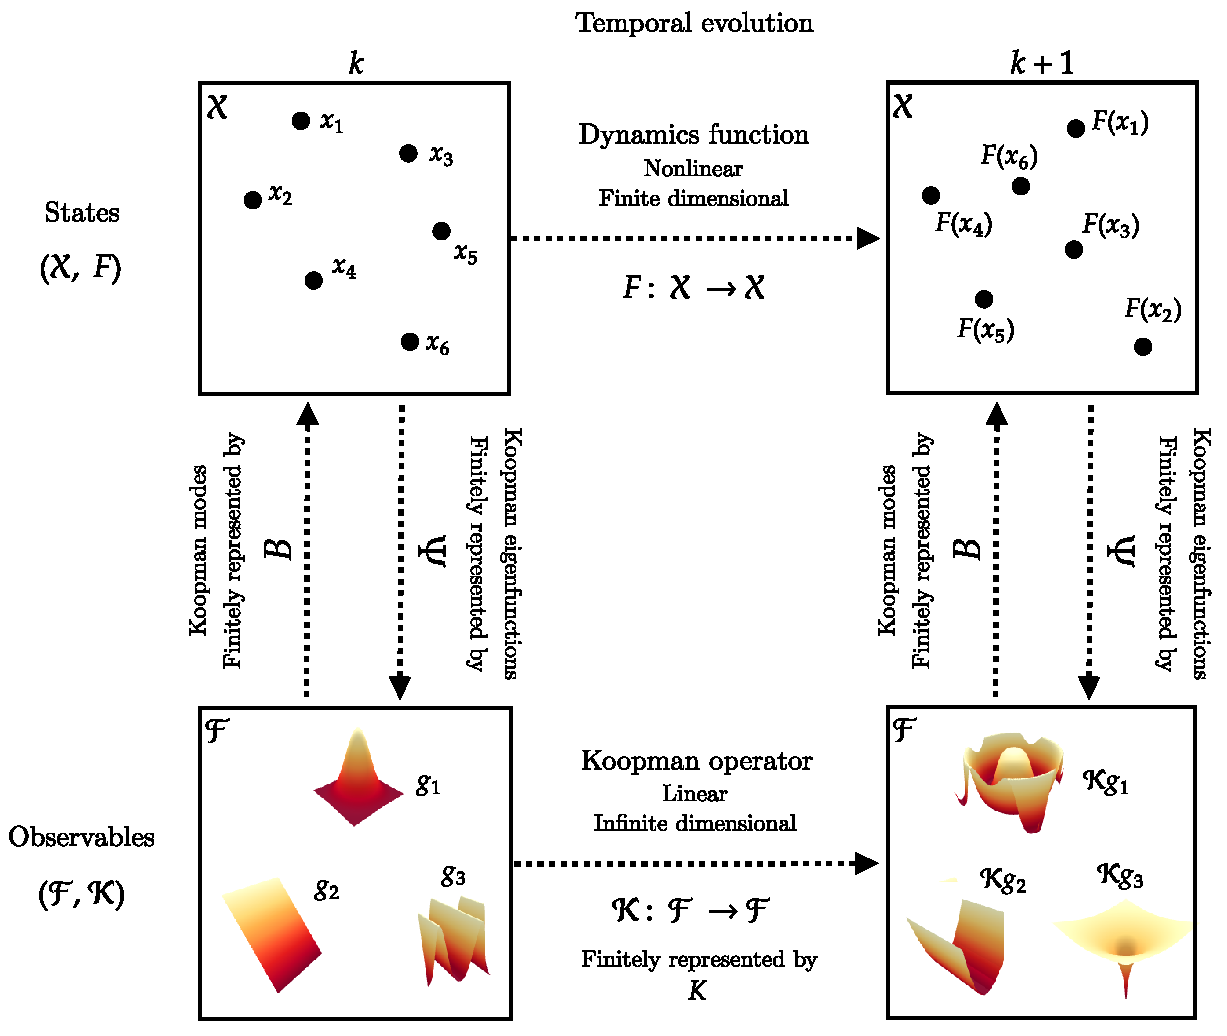
\includegraphics[scale=0.75]{img/content/chapter2/KoopDiag.pdf}
\caption{Diagrama de evolución temporal en dimensión infinita y finita, representando la dinámica mediante el operador de Koopman y sus aproximaciones. Elaboración propia, basado en \cite{Williams2015ADecomposition}.}
\label{fig:KoopDiag}
\end{figure}

\section{Aproximación de rango bajo de matrices}
La dimensión de aproximación del operador de Koopman puede ser muy alta para ciertas aplicaciones, lo que hace que ciertas operaciones se hagan muy inestables si se mantiene el rango original. Es por ello que en muchos contextos se propone bajar el rango de las matrices involucradas vía Descomposición en Valores Singulares (SVD). \\
Primero consideremos el problema de obtener la mejor matriz de rango bajo que aproxima otra matriz dada. La solución de este problema fue dada en \cite{Eckart1936TheRank}, para ello se denota por $r(\mathbf{A})$ el rango de una matriz $\mathbf{A} \in \R^{m \times n}$.

\begin{lema}
	La mejor aproximación de rango \( s \), en términos de la norma de Frobenius, para una matriz \( \mathbf{A} \) de rango \( t \) con \( t \geq s \), es decir, un minimizador global \( \hat{\mathbf{A}}^* \) de
	\[
	\min_{\hat{\mathbf{A}}} \| \mathbf{A} - \hat{\mathbf{A}} \|_F, \quad \text{s.a.} \quad r(\hat{\mathbf{A}}) \leq s
	\]
	viene dada por
	\[
	\hat{\mathbf{A}}^* = P_s (\mathbf{A}) = \mathbf{U} \Sigma_s \mathbf{V}^T,
	\]
	donde \( \Sigma_s \) es la matriz diagonal con los \( s \) valores singulares más grandes de \( \mathbf{A} \) y luego solo $0$, en donde se denota a la SVD de \( \mathbf{A} = \mathbf{U} \Sigma \mathbf{V}^T \).
\end{lema}
\noindent Es con esto que en \cite{Xiang2012OptimalMinimization} se provee una forma cerrada para un problema de regresión lineal en el que se busca que la matriz solución sea de rango bajo también, esto se formula como
\begin{equation}
	\min_{\mathbf{M}} \| \mathbf{Y} - \mathbf{M}\mathbf{X} \|_F, \quad \text{s.a.} \quad r(\mathbf{M}) \leq s
\end{equation}
\begin{prop}
	Sea la SVD de $\mathbf{X} = \mathbf{U} \Sigma \mathbf{V}^T$, con $\textbf{U} \in \R^{m \times m}$, $\mathbf{V} \in \R^{n \times n}$ matrices ortogonales y $\Sigma$ la matriz diagonal con los valores singulares. Luego, el óptimo debe cumplir
	\[
	\mathbf{V}^T \mathbf{M}^* =
	\begin{bmatrix}
		\Sigma_{r(\mathbf{X})}^{-1} P_s(\mathbf{W}_{r(\mathbf{X})}) \\
		\mathbf{a}
	\end{bmatrix},
	\]
	donde $\Sigma_{r(\mathbf{X})}$ es la matriz diagonal con los valores singulares no nulos de $\mathbf{X}$, $\mathbf{W}_{r(\mathbf{X})}$ aquella con las primeras $r(\mathbf{X})$ filas de $\mathbf{W}$, con $\mathbf{W} = \mathbf{U}^T \mathbf{Y}$.
\end{prop}
\noindent Este resultado será importante para poder trabajar matrices de alta dimensionalidad, como ocurre en el caso de EDMD.
